%===============================================================================
% LaTeX sjabloon voor de bachelorproef toegepaste informatica aan HOGENT
% Meer info op https://github.com/HoGentTIN/latex-hogent-report
%===============================================================================

\documentclass[dutch,dit,thesis]{hogentreport}

% TODO:
% - If necessary, replace the option `dit`' with your own department!
%   Valid entries are dbo, dbt, dgz, dit, dlo, dog, dsa, soa
% - If you write your thesis in English (remark: only possible after getting
%   explicit approval!), remove the option "dutch," or replace with "english".

%% Pictures to include in the text can be put in the graphics/ folder
\graphicspath{{../graphics/}}

%% For source code highlighting, requires pygments to be installed
%% Compile with the -shell-escape flag!
\usepackage[chapter]{minted}
%% If you compile with the make_thesis.{bat,sh} script, use the following
%% import instead:
% \usepackage[chapter,outputdir=../output]{minted}
% \usemintedstyle{solarized-light}

%% Formatting for minted environments.
\setminted{%
    autogobble,
    frame=lines,
    breaklines,
    linenos,
    tabsize=4
}

%% Ensure the list of listings is in the table of contents
\renewcommand\listoflistingscaption{%
    \IfLanguageName{dutch}{Lijst van codefragmenten}{List of listings}
}
\renewcommand\listingscaption{%
    \IfLanguageName{dutch}{Codefragment}{Listing}
}
\renewcommand*\listoflistings{%
    \cleardoublepage\phantomsection\addcontentsline{toc}{chapter}{\listoflistingscaption}%
    \listof{listing}{\listoflistingscaption}%
}

% Other packages not already included can be imported here

%%---------- Document metadata -------------------------------------------------
% TODO: Replace this with your own information
\author{Maarten Van der Schueren}
\supervisor{Dhr. M. Saelens}
\cosupervisor{Dhr. B. Peirens}
\title[]%
    {Toepassen van een tijdelijke grafiek transformatie op object traceringsdata voor het trainen van een LLM}
\academicyear{\advance\year by -1 \the\year--\advance\year by 1 \the\year}
\examperiod{1}
\degreesought{\IfLanguageName{dutch}{Professionele bachelor in de toegepaste informatica}{Bachelor of applied computer science}}
\partialthesis{false} %% To display 'in partial fulfilment'
\institution{Tracked N.V.}

%% Add global exceptions to the hyphenation here
\hyphenation{back-slash}

%% The bibliography (style and settings are  found in hogentthesis.cls)
\addbibresource{bachproef.bib}           %% Bibliography file
\addbibresource{../voorstel/voorstel.bib} %% Bibliography research proposal
\defbibheading{bibempty}{}

%% Prevent empty pages for right-handed chapter starts in twoside mode
\renewcommand{\cleardoublepage}{\clearpage}

\renewcommand{\arraystretch}{1.2}

%% Content starts here.
\begin{document}

%---------- Front matter -------------------------------------------------------

\frontmatter

\hypersetup{pageanchor=false} %% Disable page numbering references
%% Render a Dutch outer title page if the main language is English
\IfLanguageName{english}{%
    %% If necessary, information can be changed here
    \degreesought{Professionele Bachelor toegepaste informatica}%
    \begin{otherlanguage}{dutch}%
       \maketitle%
    \end{otherlanguage}%
}{}

%% Generates title page content
\maketitle
\hypersetup{pageanchor=true}

%%=============================================================================
%% Voorwoord
%%=============================================================================

\chapter*{\IfLanguageName{dutch}{Woord vooraf}{Preface}}%
\label{ch:voorwoord}

%% TODO:
%% Het voorwoord is het enige deel van de bachelorproef waar je vanuit je
%% eigen standpunt (``ik-vorm'') mag schrijven. Je kan hier bv. motiveren
%% waarom jij het onderwerp wil bespreken.
%% Vergeet ook niet te bedanken wie je geholpen/gesteund/... heeft
In deze bachelorproef heb ik me verdiept in het ontwikkelen van een oplossing waarmee we met behulp van een chatbot en grafiekmodellering efficiënt kunnen achterhalen waar in het staalproces van ArcelorMittal een mogelijke fout is ontstaan. 
Dit staalproces is een complex stappenplan waarbij het staal begint bij grondstoffen die in de fabriek aankomen en eindigen als een afgewerkt product dat naar de klant wordt verzonden.
Het doel van dit onderzoek is om een methode te vinden die het mogelijk maakt snel en accuraat processen te identificeren en eventuele foutmeldingen te detecteren.
Door een vraag te stellen aan de chatbot, gaat deze op zoek naar mogelijke knelpunten in het proces. Daarna verwachten we dat de chatbot dit in een duidelijk antwoord kan uitleggen op basis van de gegevens uit de database.
Dit onderzoek voer ik uit in samenwerking met mijn co-promotor Bart Peirens van Tracked, die ons ondersteunt bij het traceerproces. Daarnaast zal Tim De Grave, software architect binnen ArcelorMittal Gent de benodigde data en resources aanleveren waarmee we deze oplossing kunnen verwezelijken. 
Ik wil hen beiden hartelijk bedanken voor hun waardevolle bijdragen en ondersteuning gedurende dit project. Verder wil ik Martijn Saelens, mijn promotor, bedanken voor de begeleiding en het vertrouwen dat hij me gegeven heeft tijdens dit proces.

%%=============================================================================
%% Samenvatting
%%=============================================================================

% TODO: De "abstract" of samenvatting is een kernachtige (~ 1 blz. voor een
% thesis) synthese van het document.
%
% Een goede abstract biedt een kernachtig antwoord op volgende vragen:
%
% 1. Waarover gaat de bachelorproef?
% 2. Waarom heb je er over geschreven?
% 3. Hoe heb je het onderzoek uitgevoerd?
% 4. Wat waren de resultaten? Wat blijkt uit je onderzoek?
% 5. Wat betekenen je resultaten? Wat is de relevantie voor het werkveld?
%
% Daarom bestaat een abstract uit volgende componenten:
%
% - inleiding + kaderen thema
% - probleemstelling
% - (centrale) onderzoeksvraag
% - onderzoeksdoelstelling
% - methodologie
% - resultaten (beperk tot de belangrijkste, relevant voor de onderzoeksvraag)
% - conclusies, aanbevelingen, beperkingen
%
% LET OP! Een samenvatting is GEEN voorwoord!

%%---------- Nederlandse samenvatting -----------------------------------------
%
% TODO: Als je je bachelorproef in het Engels schrijft, moet je eerst een
% Nederlandse samenvatting invoegen. Haal daarvoor onderstaande code uit
% commentaar.
% Wie zijn bachelorproef in het Nederlands schrijft, kan dit negeren, de inhoud
% wordt niet in het document ingevoegd.

\IfLanguageName{english}{%
\selectlanguage{dutch}
\chapter*{Samenvatting}

\selectlanguage{english}
}{}

%%---------- Samenvatting -----------------------------------------------------
% De samenvatting in de hoofdtaal van het document

\chapter*{\IfLanguageName{dutch}{Samenvatting}{Abstract}}




%---------- Inhoud, lijst figuren, ... -----------------------------------------

\tableofcontents

% In a list of figures, the complete caption will be included. To prevent this,
% ALWAYS add a short description in the caption!
%
%  \caption[short description]{elaborate description}
%
% If you do, only the short description will be used in the list of figures

\listoffigures

% If you included tables and/or source code listings, uncomment the appropriate
% lines.
\listoftables

\listoflistings

% Als je een lijst van afkortingen of termen wil toevoegen, dan hoort die
% hier thuis. Gebruik bijvoorbeeld de ``glossaries'' package.
% https://www.overleaf.com/learn/latex/Glossaries

%---------- Kern ---------------------------------------------------------------

\mainmatter{}

% De eerste hoofdstukken van een bachelorproef zijn meestal een inleiding op
% het onderwerp, literatuurstudie en verantwoording methodologie.
% Aarzel niet om een meer beschrijvende titel aan deze hoofdstukken te geven of
% om bijvoorbeeld de inleiding en/of stand van zaken over meerdere hoofdstukken
% te verspreiden!

%%=============================================================================
%% Inleiding
%%=============================================================================

\chapter{\IfLanguageName{dutch}{Inleiding}{Introduction}}%
\label{ch:inleiding}

In de moderne industriële wereld is efficiëntie en performantie cruciaal, vooral binnen ingewikkelde toeleveringsketens zoals die van ArcelorMittal Gent. 
Deze bachelorproef richt zich op het verbeteren van klachtenafhandeling en preventie van fouten, door gebruik te maken van innovatieve technologieën zoals grafiekmodellering en large language models (LLMs). 
Door traceringsdata om te zetten naar een grafiekmodel en dit te koppelen aan een LLM, kunnen bedrijven in staat gesteld worden om sneller en nauwkeuriger de oorzaken van problemen te achterhalen. 

Dit onderzoek, uitgevoerd in samenwerking met Tracked, een bedrijf van de Cronos groep gespecialiseerd in traceringsdata, heeft als doel om schaalbare en performante oplossingen te bieden die de efficiëntie en klanttevredenheid optimaliseren.
Voor dit onderzoek maken we gebruik van een installatieboom die alle onderdelen van het productieproces bevat.

Let op dat de data die we gebruiken omtrent dit proces louter fictief is en enkel dient ter illustratie van de werking van de verschillende technologieën.
In~\ref{sec:dataopstelling} wordt er meer uitleg gegeven over de data die we gebruiken aangezien we niet de originele data hebben gebruikt om dit onderzoek te volbrengen.
De reden hiervoor is dat de originele data vertrouwelijk is en niet openbaar kan worden gemaakt. 
Daarnaast is er ook gevraagd om een minim aantal code weer te geven in de thesis, dit om de data zo confidentieel mogelijk te houden.

\section{\IfLanguageName{dutch}{Probleemstelling}{Problem Statement}}%
\label{sec:probleemstelling}

% Uit je probleemstelling moet duidelijk zijn dat je onderzoek een meerwaarde heeft voor een concrete doelgroep. De doelgroep moet goed gedefinieerd en afgelijnd zijn. Doelgroepen als ``bedrijven,'' ``KMO's'', systeembeheerders, enz.~zijn nog te vaag. Als je een lijstje kan maken van de personen/organisaties die een meerwaarde zullen vinden in deze bachelorproef (dit is eigenlijk je steekproefkader), dan is dat een indicatie dat de doelgroep goed gedefinieerd is. Dit kan een enkel bedrijf zijn of zelfs één persoon (je co-promotor/opdrachtgever).
In de complexe toeleveringsketen van ArcelorMittal Gent zijn er veel verschillende processen die verspreid zijn over meerdere afdelingen. 
Deze processen omvatten onder andere de productie, verpakking en logistiek.
Elke afdeling heeft specifieke processen en datamodellen, wat het analyseren en onderzoeken van gegevens over afdelingen heen zeer complex en tijdrovend maakt. 
Dit leidt tot inefficiënties in de klachtenafhandeling of onderhoudsprocessen, en verhoogt de operationele kosten. 
Er is behoefte aan een schaalbare en performante oplossing die bedrijven in staat stelt sneller en nauwkeuriger de oorzaken van problemen te achterhalen, waardoor duur en tijdrovend handmatig werk wordt verminderd.
Dit is een erkend probleem voor zowel kleine bedrijven (zoals bijvoorbeeld kleine ondernemingen) en zeker bij grote bedrijven (zoals in dit geval ArcelorMittal), waarbij het staal een grote weg aflegt en niet alleen in Gent blijft.
Dit staal wordt namelijk geproduceerd, verwerkt en gebruikt in verschillende regio's, daarnaast zijn er ook verschillende logistieke middelen die het staal vervoeren naar de klant (zoals een boot, trein of vrachtwagen).
\section{\IfLanguageName{dutch}{Onderzoeksvraag}{Research question}}%
\label{sec:onderzoeksvraag}

% Wees zo concreet mogelijk bij het formuleren van je onderzoeksvraag. Een onderzoeksvraag is trouwens iets waar nog niemand op dit moment een antwoord heeft (voor zover je kan nagaan). Het opzoeken van bestaande informatie (bv. ``welke tools bestaan er voor deze toepassing?'') is dus geen onderzoeksvraag. Je kan de onderzoeksvraag verder specifiëren in deelvragen. Bv.~als je onderzoek gaat over performantiemetingen, dan 
De voornaamste onderzoeksvraag luidt als volgt: \emph{`Hoe kunnen we efficiënt en snel grafiekmodellering toepassen en met behulp van een large language model (LLM) een chatbot ontwikkelen die in staat is om het waar, wanneer, wat en hoe van gebeurtenissen binnen een proces vast te stellen ter ondersteuning van klachtenafhandeling bij productfouten\texttt{?}}`

Daarnaast zijn belangrijke deelvragen:
\begin{itemize}
    \item Hoe kunnen we SAP-data omzetten naar een grafiekmodel?
    \item Hoe maken we gebruik van de GS1 standaarden om de data correct te structureren?
    \item Hoe kunnen we een LLM gebruiken om gebeurtenissen binnen een proces vast te stellen?
    \item Hoe kunnen we een chatbot ontwikkelen die een LLM kan bevragen en een gepast antwoord kan geven op de gestelde vraag?
\end{itemize}
\section{\IfLanguageName{dutch}{Onderzoeksdoelstelling}{Research objective}}%
\label{sec:onderzoeksdoelstelling}

% Wat is het beoogde resultaat van je bachelorproef? Wat zijn de criteria voor succes? Beschrijf die zo concreet mogelijk. Gaat het bv.\ om een proof-of-concept, een prototype, een verslag met aanbevelingen, een vergelijkende studie, enz.
De doelstelling van deze bachelorproef is om een schaalbare en performante oplossing te ontwikkelen die bedrijven in staat stelt sneller en nauwkeuriger de oorzaken van problemen binnen hun toeleveringsketen te achterhalen.
Dit wordt bereikt door het toepassen van grafiekmodellering op traceringsdata en het gebruiken van een large language model (LLM). 
Het uiteindelijke doel is om de operationele efficiëntie te verbeteren en de klanttevredenheid te optimaliseren door een efficiënte klachtenafhandeling mogelijk te maken.

Binnen de doelstelling van deze bachelorproef wordt er nogmaals benadrukt dat er gebruik gemaakt wordt van fictieve data gebasseerd op de boomstructuur van ArcelorMittal waarbij alle afdelingen en werktuigen staan opgelijst. 
Daarbij is het doel dat we kunnen vragen: \emph{``Geef alle machines met een alarm op de motor.''}, en dat de chatbot dit kan beantwoorden.

\section{Databeschrijving vooraf}\label{sec:dataopstelling}
Vooraleer er aan de slag gegaan wordt met deze bachelorproef, is het belangrijk om te weten welke data precies beschikbaar is en hoe die eruitziet.

Aan het begin van deze thesis werd er een SAP-boomstructuur in JSON-formaat aangeleverd, die alle onderdelen van het productieproces bevat.
Dit bestand is enorm groot (meer dan 50.000 JSON-objecten) en bevat bovendien een groot aantal eigenschappen per object.
Door deze complexiteit is het moeilijk om meteen met de volledige dataset te werken tijdens de ontwikkeling van de chatbot.

Om sneller te kunnen testen en ontwikkelen, wordt er daarom gekozen voor een mock dataset.
Deze heeft dezelfde structuur als de originele data, maar maakt gebruik van fictieve sleutel-waarde paren en een veel kleiner aantal records.
Hierdoor kan de initiële opzet en het testen uitgevoerd worden zonder dat telkens de volledige dataset moet worden ingeladen.

Voor de verdere ontwikkeling van het project maakt het geen verschil of de mock-data of de echte data wordt gebruikt.
De scripts in zowel JavaScript als Python zijn generiek opgebouwd en functioneren zolang de datastructuur ongewijzigd blijft.

Doorgaans start het proces met een JSON-bestand dat via een Python-script wordt omgezet naar JSON-LD.\@
Dit JSON-LD-bestand kan vervolgens rechtstreeks in Cosmos DB worden ingeladen.

In figuur~\ref{fig:graphmodel} is een voorbeeld te zien van hoe de mock-data eruitziet in grafiekvorm.

\section{\IfLanguageName{dutch}{Opzet van deze bachelorproef}{Structure of this bachelor thesis}}%
\label{sec:opzet-bachelorproef}

% Het is gebruikelijk aan het einde van de inleiding een overzicht te
% geven van de opbouw van de rest van de tekst. Deze sectie bevat al een aanzet
% die je kan aanvullen/aanpassen in functie van je eigen tekst.
De bachelorproef is als volgt opgebouwd:

Eerst en vooral, in hoofdstuk~\ref{ch:stand-van-zaken} wordt er een overzicht gegeven over welke technologieën hiervoor gebruikt zijn.
Daarnaast wordt er ook een overzicht gegeven van de literatuur die relevant is voor dit onderzoek.

Daarna wordt er in hoofdstuk~\ref{ch:methodologie} de methodologie toegelicht en worden de gebruikte onderzoekstechnieken besproken om een antwoord te kunnen formuleren op de onderzoeksvragen.
Zo wordt besproken hoe de SAP-data kan worden omgezet naar een grafiekmodel, waarom er gebruik wordt gemaakt van een LLM en hoe deze wordt geïmplementeerd via een REST-API.\@
Dit alles wordt opgebouwd in Docker om flexibel te zijn met de onderliggende infrastructuur, waardoor de chatbot eenvoudig kan worden beheerd.

% TODO: Vul hier aan voor je eigen hoofstukken, één of twee zinnen per hoofdstuk

Tot slot, in hoofdstuk~\ref{ch:conclusie}, wordt er een antwoord geformuleerd op de onderzoeksvragen en geven we een conclusie over deze thesis. Daarnaast worden een aantal mogelijke uitbereidingen voor dit onderzoek besproken.


Indien er gerefereerd wordt naar een bijlage, maar verder geen uitleg over gegeven wordt, kan je die bijlage vinden in hoofdstuk~\ref{ch:Bijlagen}.
\chapter{\IfLanguageName{dutch}{Stand van zaken}{State of the art}}%
\label{ch:stand-van-zaken}

% Tip: Begin elk hoofdstuk met een paragraaf inleiding die beschrijft hoe
% dit hoofdstuk past binnen het geheel van de bachelorproef. Geef in het
% bijzonder aan wat de link is met het vorige en volgende hoofdstuk.

% Pas na deze inleidende paragraaf komt de eerste sectiehoofding.

% Dit hoofdstuk bevat je literatuurstudie. De inhoud gaat verder op de inleiding, maar zal het onderwerp van de bachelorproef *diepgaand* uitspitten. De bedoeling is dat de lezer na lezing van dit hoofdstuk helemaal op de hoogte is van de huidige stand van zaken (state-of-the-art) in het onderzoeksdomein. Iemand die niet vertrouwd is met het onderwerp, weet nu voldoende om de rest van het verhaal te kunnen volgen, zonder dat die er nog andere informatie moet over opzoeken \autocite{Pollefliet2011}.

% Je verwijst bij elke bewering die je doet, vakterm die je introduceert, enz.\ naar je bronnen. In \LaTeX{} kan dat met het commando \texttt{$\backslash${textcite\{\}}} of \texttt{$\backslash${autocite\{\}}}. Als argument van het commando geef je de ``sleutel'' van een ``record'' in een bibliografische databank in het Bib\LaTeX{}-formaat (een tekstbestand). Als je expliciet naar de auteur verwijst in de zin (narratieve referentie), gebruik je \texttt{$\backslash${}textcite\{\}}. Soms is de auteursnaam niet expliciet een onderdeel van de zin, dan gebruik je \texttt{$\backslash${}autocite\{\}} (referentie tussen haakjes). Dit gebruik je bv.~bij een citaat, of om in het bijschrift van een overgenomen afbeelding, broncode, tabel, enz. te verwijzen naar de bron. In de volgende paragraaf een voorbeeld van elk.

% \textcite{Knuth1998} schreef een van de standaardwerken over sorteer- en zoekalgoritmen. Experten zijn het erover eens dat cloud computing een interessante opportuniteit vormen, zowel voor gebruikers als voor dienstverleners op vlak van informatietechnologie~\autocite{Creeger2009}.

% Let er ook op: het \texttt{cite}-commando voor de punt, dus binnen de zin. Je verwijst meteen naar een bron in de eerste zin die erop gebaseerd is, dus niet pas op het einde van een paragraaf.

\label{sec:grafiekmodellering}
\section{Grafiekmodellering}
Grafiekmodellering is een techniek die gebruikt wordt om de data te visualiseren en te analyseren. In deze bachelorproef wordt dit gebruikt om de verbanden te leggen tussen de verschillende processen binnen ArcelorMittal Gent.
Dit gebeurt door middel van knopen die verbonden zijn met edges, welke de relaties tussen de verschillende knopen weergeven \autocite{neo4j2025}.
Een knoop stelt een entiteit voor, zoals een persoon, een product of een proces. Een edge stelt de relatie tussen de verschillende knopen voor zoals een associatie, transformatie of transactie van een product.
Dit kan in ons geval een staalplaat zijn die door een kraan verplaatst wordt. Hierbij zijn de kraan en staalplaat de knopen en is de verplaatsing een transactie-relatie tussen deze knopen.
Elke knoop bevat ook properties die de knoop beschrijven. Dit kan bijvoorbeeld het bouwjaar van een machine zijn of de temperatuur van een product, deze worden opgeslagen als key-value paar om later efficiënt te kunnen ophalen.

\subsection{Cosmos DB}%
Cosmos DB is een NoSQL\-database van Microsoft. Het biedt een lage latentie, multi\-query-API die eenvoudig grote hoeveelheden data kan verwerken en heeft een grote beschikbaarheid zegt~\textcite{Put2020}, wat zeer belangrijk is in ons project.
Daarnaast is CosmosDB horizontaal schaalbaar, wat betekent dat we op hoogtepunten tot een miljoen lees- en schrijfaanvragen kunnen verwerken door het benodigde aantal servers toe te voegen.
De hoge beschikbaarheid wordt gegarandeerd door replicatie, waardoor we snel kunnen overschakelen als er een probleem is in onze database.
Binnen ArcelorMittal wordt gebruik gemaakt van de azure omgeving van Microsoft, waardoor CosmosDB een logische keuze is voor ons project.
CosmosDB ondersteunt verschillende API's zoals SQL, MongoDB, Cassandra, Gremlin en Table API, waardoor we flexibel kunnen werken met verschillende soorten data.

\subsection{Gremlin API}
Gremlin is een database query taal die gebruikt wordt om te communiceren met grafiek databases zoals CosmosDB \autocite{Tinkerpop2023}.\@
De taal bevat verschillende varianten zoals Gremlin-Java, Gremlin-Python en Gremlin-Groovy,\dots
In ons geval zullen we Gremlin-Javascript gebruiken om de data van ArcelorMittal Gent in CosmosDB te bevragen. De bevraging is gebasseerd op een RestAPI die de data ophaalt en teruggeeft in json formaat.
Javascript is hiervoor geschikt omdat Javascript en json een goede combinatie zijn om data te verwerken, daarnaast maken we ook gebruik van nodejs wat met javascript werkt. 
Als extra kan je met javascript eenvoudig front end en back end combineren, wat mogelijk is voor verdere uitbereiding van deze thesis.
Hiernaast hebben we ook Neo4J overwogen met cypher als query taal, maar deze heeft zijn eigen ecosysteem en is niet even flexibel en schaalbaar als Gremlin.
Gremlin daarentegen voorziet dat alle databases die TinkerPop-enabled zijn, kunnen worden gebruikt. Hieronder vallen onder andere Amazon Neptune, CosmosDB, JanusGraph en nog vele andere.\autocite{Tinkerpop2023a}

\subsection{NodeJS}
NodeJS is een open-source JavaScript runtime-omgeving die de mogelijkheid biedt om JavaScript-code uit te voeren op de server \autocite{NodeJS2022}.
Dit gebeurt Single\-Threaded, Non\-Blocking I/O model wat betekent dat er geen nieuwe threads worden aangemaakt voor elke request.
Door middel van Callbacks en Promises werkt nodejs asynchroon, wat betekent dat de code niet wacht op een antwoord van een request maar ondertussen andere requests kan verwerken.
Met event loops worden de requests in een wachtrij geplaatst en worden ze verwerkt wanneer de server klaar is met een andere operatie.
Daardoor is NodeJS zeer performant en schaalbaar voor het verwerken van grote hoeveelheden data.

De tecnologie is in 2009 ontwikkeld en geintroceerd door Ryan Dahl en is sindsdien zeer populair geworden in de webontwikkeling. 
NodeJS is later door grote bedrijven zoals Netfilx, eBay \& Uber gebruikt voor hun back-end systemen.
Zoals eerder vermeld is het geen framework maar een runtime-omgeving, dit betekent dat het geen standaardbibliotheken heeft die hergebruikt kunnen worden door developers.
Daardoor ben je volledig vrij in hoe je de architectuur van je applicatie opbouwt.

Een van de nadelen van nodejs is dat het single\-threaded is, wat betekent dat het niet geschikt is voor CPU-intensieve taken.
Dit komt omdat nodejs gebruik maakt van een event loop die de requests in een wachtrij plaatst en ze verwerkt wanneer de server klaar is met een andere operatie.
Hierdoor kan het zijn dat een request die veel tijd nodig heeft om te verwerken de andere requests blokkeert.
Sinds 2018 is er een nieuwe feature geïntroduceerd in nodejs genaamd Worker Threads, dit maakt het mogelijk om multi\-threaded te werken in nodejs.
Daardoor kunnen we de CPU\-intensieve taken in een aparte thread verwerken en de main thread vrij houden voor andere requests.

\subsection{EPCIS}
Voor dit onderzoek maken we gebruik van EPCIS (Electronic Product Code Information Services) waarden voor de producten, dit zijn de wat, wanneer, waar, waarom en hoe. 
Deze waarden zijn ontwikkeld door GS1 om gegevens over beweging, status en verandering van een item in de toeleveringsketen (supply chain) vast te leggen en te delen binnen en buiten het bedrijf \autocite{Devins}.
``Met behulp van deze waarden kunnen we real-life objecten omzetten in elektronisch opgeslagen informatie, waarna we dit kunnen communiceren met eindgebruikers.`` zegt \textcite{Devins}.
Door deze normen toe te passen kunnen we de traceerbaarheid van het product per proces garanderen inclusief de gewenste parameters die opgeslagen worden in ons grafiekmodel zoals tijd (wanneer) en temperatuur (hoe) waar nodig.
EPCIS is een GS1-standaard die bedrijven in staat stelt om gebeurtenissen in de toeleveringsketen vast te leggen en te delen. Het biedt een gemeenschappelijk kader voor het vastleggen van de wat, wanneer, waar en waarom van gebeurtenissen die betrekking hebben op fysieke of digitale objecten. Dit helpt bedrijven om een gedetailleerd overzicht te krijgen van de bewegingen en status van producten in de toeleveringsketen, wat essentieel is voor traceerbaarheid en transparantie.

Volgens GS1 \autocite{GS12025} zijn de belangrijkste voordelen van EPCIS:
\begin{table}[H]
    \centering
     \begin{tabular}{lp{0.6\textwidth}}
          \toprule
          \textbf{Voordeel} & \textbf{Beschrijving} \\
          \toprule
          Verbeterde zichtbaarheid & Door het vastleggen en delen van gedetailleerde gebeurtenisgegevens kunnen bedrijven beter inzicht krijgen in de bewegingen en status van producten in de toeleveringsketen. \\
          \midrule
          Efficiëntieverbeteringen & Door het automatiseren van gegevensverzameling en -uitwisseling kunnen bedrijven operationele efficiëntie verbeteren en fouten verminderen. \\
          \midrule
          Naleving van regelgeving & EPCIS helpt bedrijven te voldoen aan wettelijke vereisten voor traceerbaarheid en rapportage. \\
          \midrule
          Betere samenwerking & Door het delen van gebeurtenisgegevens met handelspartners kunnen bedrijven beter samenwerken en de toeleveringsketen optimaliseren. \\
          \bottomrule
     \end{tabular}
     \caption[Belangrijkste voordelen van EPCIS volgens GS1]{\label{tab:epcis-voordelen}}
\end{table}

Door EPCIS te implementeren in ons project kunnen we ervoor zorgen dat alle relevante gegevens over de beweging en status van producten nauwkeurig worden vastgelegd en gedeeld, wat bijdraagt aan een efficiëntere en transparantere toeleveringsketen.

\section{Data preprocessing}
De data die we gebruiken komt uit een SAP systeem. Deze data bevat een functionele boom structuur van de verschillende levels binnen ArcelorMittal Gent.
Dit houdt in dat de data in een hiërarchische structuur is opgebouwd, waarbij de verschillende processen met elkaar verbonden zijn.
Voor het ontcijferen van deze data hebben we verschillende specialisten binnen ArcelorMittal gecontacteerd die ons hebben geholpen met het vertalen van de datacodes.
Zo zijn we te weten gekomen dat level 1 in de boom de site zelf is en dat level 2 de verschillende afdelingen zijn binnen de site. Zo gaat het telkens dieper tot level 11 waar de verschillende onderdelen van de machines zich bevinden.
Elke machine heeft een unieke code die we uit een dictionairy kunnen halen die we hebben ontvangen van ArcelorMittal.
Deze ontcijferingen zijn nodig in een later proces om onze chatbot een correct antwoord te laten geven op de vragen van de gebruiker.

\subsection{JSON tot Graph}
De data die we ontvangen van ArcelorMittal uit SAP is in json formaat. Deze data stelt ons in staat om door de beschrijving van de keywords de data te ontcijferen en te verwerken in ons grafiekmodel.
Omdat wij voor Gremlin en EPCIS werken met schema.org hebben wij een json-ld formaat nodig. Dit is een uitbreiding van json die het mogelijk maakt om data te structureren en te annoteren.
Daarna kunnen we deze json-ld in een folder plaatsen en wordt deze automatisch ingelezen met een nodejs script.
Deze gaat voor alle types een knoop aanmaken die de juiste properties bevat. Daarna kunnen we ook de edges aanmaken volgens de schema.org structuur.

\subsection{Schema.org}
Schema.org is een grote verzameling van gestructureerde data die entiteiten (knopen) en relaties kan weergeven \autocite{Douglas2023}.
Je kan schema.org vergelijken met GS1 maar dan meer generiek. In ons project zullen we de combinatie van schema.org objecten en GS1 objecten gebruiken om de data te structureren.

% \begin{figure}
%   \centering
%   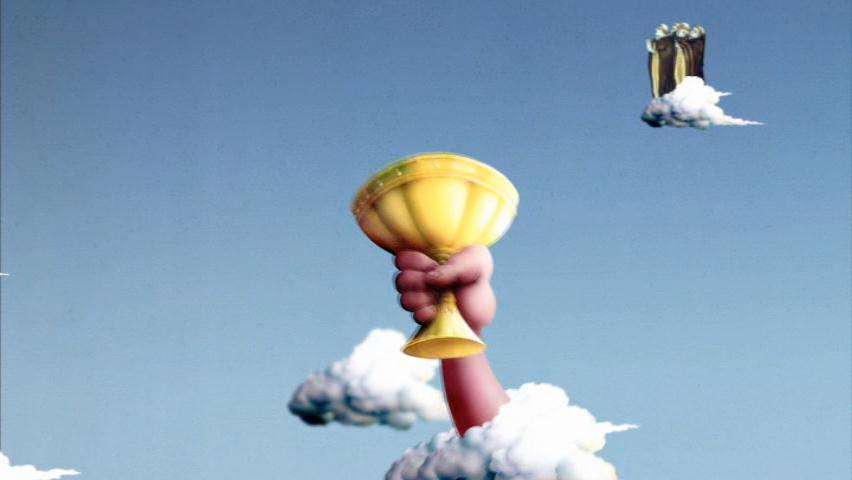
\includegraphics[width=0.8\textwidth]{grail.jpg}
%   \caption[Voorbeeld figuur.]{\label{fig:grail}Voorbeeld van invoegen van een figuur. Zorg altijd voor een uitgebreid bijschrift dat de figuur volledig beschrijft zonder in de tekst te moeten gaan zoeken. Vergeet ook je bronvermelding niet!}
% \end{figure}

% \begin{listing}
%   \begin{minted}{python}
%     import pandas as pd
%     import seaborn as sns

%     penguins = sns.load_dataset('penguins')
%     sns.relplot(data=penguins, x="flipper_length_mm", y="bill_length_mm", hue="species")
%   \end{minted}
%   \caption[Voorbeeld codefragment]{Voorbeeld van het invoegen van een codefragment.}
% \end{listing}


% \begin{table}
%   \centering
%   \begin{tabular}{lcr}
%     \toprule
%     \textbf{Kolom 1} & \textbf{Kolom 2} & \textbf{Kolom 3} \\
%     $\alpha$         & $\beta$          & $\gamma$         \\
%     \midrule
%     A                & 10.230           & a                \\
%     B                & 45.678           & b                \\
%     C                & 99.987           & c                \\
%     \bottomrule
%   \end{tabular}
%   \caption[Voorbeeld tabel]{\label{tab:example}Voorbeeld van een tabel.}
% \end{table}


%%=============================================================================
%% Methodologie
%%=============================================================================

\chapter{\IfLanguageName{dutch}{Methodologie}{Methodology}}%
\label{ch:methodologie}

%% TODO: In dit hoofstuk geef je een korte toelichting over hoe je te werk bent
%% gegaan. Verdeel je onderzoek in grote fasen, en licht in elke fase toe wat
%% de doelstelling was, welke deliverables daar uit gekomen zijn, en welke
%% onderzoeksmethoden je daarbij toegepast hebt. Verantwoord waarom je
%% op deze manier te werk gegaan bent.
%% 
%% Voorbeelden van zulke fasen zijn: literatuurstudie, opstellen van een
%% requirements-analyse, opstellen long-list (bij vergelijkende studie),
%% selectie van geschikte tools (bij vergelijkende studie, "short-list"),
%% opzetten testopstelling/PoC, uitvoeren testen en verzamelen
%% van resultaten, analyse van resultaten, ...
%%
%% !!!!! LET OP !!!!!
%%
%% Het is uitdrukkelijk NIET de bedoeling dat je het grootste deel van de corpus
%% van je bachelorproef in dit hoofstuk verwerkt! Dit hoofdstuk is eerder een
%% kort overzicht van je plan van aanpak.
%%
%% Maak voor elke fase (behalve het literatuuronderzoek) een NIEUW HOOFDSTUK aan
%% en geef het een gepaste titel.

\lipsum[21-25]



% Voeg hier je eigen hoofdstukken toe die de ``corpus'' van je bachelorproef
% vormen. De structuur en titels hangen af van je eigen onderzoek. Je kan bv.
% elke fase in je onderzoek in een apart hoofdstuk bespreken.

%\input{...}
%\input{...}
%...

%%=============================================================================
%% Conclusie
%%=============================================================================

\chapter{Conclusie}%
\label{ch:conclusie}
In deze bachelorproef werd onderzocht hoe we gebruik konden maken van een grafiekmodel en een Large Language Model (LLM) om gegevens binnen het staalproductieproces van ArcelorMittal Gent efficiënt op te vragen. 
Het doel was om een proof of concept te ontwikkelen die niet alleen de traceerbaarheid van productieprocessen verbetert, maar ook de operationele efficiëntie verhoogt door middel van een chatbot die procesvragen kan beantwoorden.
Door de SAP boomstructuur om te zetten naar een JSON-LD formaat volgens GS1-standaarden, en deze te structureren in een grafiekdatabase (CosmosDB), werd een stevige basis gelegd voor het traceren van productieprocessen.
Vervolgens werd een chatbot ontwikkeld die gebruik maakt van Gremlin queries en Retrieval Augmented Generation (RAG) om procesvragen te vertalen naar begrijpelijke antwoorden.
Door gebruik te maken van modellen zoals Code Llama voor querygeneratie en Phi-4 voor natuurlijke taalverwerking, kon een performante oplossing worden opgezet die uit te bereiden is en bruikbaar voor andere use-cases binnen de industrie.

In dit ondezoek ben ik vooral op zoek gegaan naar combinaties van technieken die het mogelijk maken om de traceerbaarheid van productieprocessen te verbeteren.
De proof of concept die werd ontwikkeld, toont aan dat het mogelijk is om een chatbot te creëren die vragen kan beantwoorden over productieprocessen door gebruik te maken van dit grafiekmodel en een LLM.\@
Mits de juiste finetuning en eventuele hertraining van de modellen, kan deze oplossing verder worden uitgebreid en geoptimaliseerd voor andere toepassingen binnen de industrie.
Naast de technische aspecten, is het ook belangrijk om de gebruikerservaring in overweging te nemen.
De chatbot is een API die kan worden geïntegreerd in bestaande systemen, waardoor het voor gebruikers eenvoudig is om toegang te krijgen tot de informatie die ze nodig hebben.
De proof of concept biedt een solide basis voor verdere ontwikkeling en implementatie binnen ArcelorMittal Gent en mogelijk ook andere bedrijven in de staalindustrie.
Naast het opzetten van een frontend, kan er ook gekeken worden naar het maken van een gremlin specifieke LLM die getrained wordt met LoRA op de mogelijke syntax van gremlin queries.
In deze thesis hebben we daar niet de tijd en resources voor gehad, maar het lijkt ons een interessante richting om verder te onderzoeken.

% TODO: Trek een duidelijke conclusie, in de vorm van een antwoord op de
% onderzoeksvra(a)g(en). Wat was jouw bijdrage aan het onderzoeksdomein en
% hoe biedt dit meerwaarde aan het vakgebied/doelgroep? 
% Reflecteer kritisch over het resultaat. In Engelse teksten wordt deze sectie
% ``Discussion'' genoemd. Had je deze uitkomst verwacht? Zijn er zaken die nog
% niet duidelijk zijn?
% Heeft het onderzoek geleid tot nieuwe vragen die uitnodigen tot verder 
%onderzoek?




%---------- Bijlagen -----------------------------------------------------------

\appendix

\chapter{Onderzoeksvoorstel}

Het onderwerp van deze bachelorproef is gebaseerd op een onderzoeksvoorstel dat vooraf werd beoordeeld door de promotor. Dat voorstel is opgenomen in deze bijlage.

%% TODO: 
\section*{Samenvatting}
    In deze bachelorproef onderzoeken we hoe grafiekmodellering kan bijdragen aan efficiënte klachtenafhandeling binnen bedrijfsprocessen. 
    Door gebruik te maken van een large language model (LLM) gekoppeld aan een chatbot willen we bedrijven in staat stellen sneller en nauwkeuriger de oorzaken van problemen te achterhalen, waardoor kostbaar handmatig werk wordt verminderd. 
    Dit door een vraag te stellen aan de chatbot waarbij hij via het grafiekmodel een ongewone gebeurtenis kan ophalen. Het onderzoek richt zich op twee fases: de omzetting van EPCIS-events naar een grafiekmodel in Cosmos DB met behulp van de Gremlin API, en het trainen van een LLM om te analyseren waar, wanneer, wat en hoe gebeurtenissen plaatsvinden. 
    Dit proces helpt bij het opsporen van anomalieën, met als doel schaalbare en performante oplossingen te bieden voor bedrijfs- en nationale use cases. 
    Uiteindelijk streven we naar het optimaliseren van klantenervaring en operationele efficiëntie.

% Kopieer en plak hier de samenvatting (abstract) van je onderzoeksvoorstel.

% Verwijzing naar het bestand met de inhoud van het onderzoeksvoorstel
%---------- Inleiding ---------------------------------------------------------

% TODO: Is dit voorstel gebaseerd op een paper van Research Methods die je
% vorig jaar hebt ingediend? Heb je daarbij eventueel samengewerkt met een
% andere student?
% Zo ja, haal dan de tekst hieronder uit commentaar en pas aan.

%\paragraph{Opmerking}

% Dit voorstel is gebaseerd op het onderzoeksvoorstel dat werd geschreven in het
% kader van het vak Research Methods dat ik (vorig/dit) academiejaar heb
% uitgewerkt (met medesturent VOORNAAM NAAM als mede-auteur).
% 

\section{Inleiding}%
\label{sec:inleiding}

Binnen de Arcelor Mittal Gent bestaan er veel verschillende processen die verdeeld zijn over verschillende afdelingen.
Iedere afdeling heeft een deel van het proces om van grondstof tot een afgewerkt product te raken. 
Hierbij is het zo dat tussen iedere afdeling een deel is van de toeleveringsketting waarbij het resultaat van de ene afdeling de start is van de andere afdeling.
Waarbij dat iedere stap zijn invloed kan hebben op de kwaliteit van het eindresultaat.

Iedere afdeling is gemaakt rond een specifiek proces zoals hoogoven die van ruwe grondstoffen naar ruw ijzer gaat en de staalfabriek die van ruw ijzer naar staal gaat.
Omdat deze afdelingen zeer specifieke processen hebben, hebben ze ook zeer specifieke noden en datamodellen.
Dit zorgt ervoor dat analyse of onderzoek over afdelingen heen zeer complex wordt en tijdsrovend is.

De scope van deze bachelorproef bestaat is tweedelig waarbij deel één eruit bestaat om samen met Tracked vanuit een gestandariseerd datamodel die zichtbaarheid events bijhoudt om te zetten naar een graphmodel.
Deel twee bouwt verder op dit graphmodel om dan een LLM te trainen om eenvoudig informatie hieruit te krijgen en terug te geven.
%---------- Stand van zaken ---------------------------------------------------

\section{Literatuurstudie}%
\label{sec:literatuurstudie}

Hier beschrijf je de \emph{state-of-the-art} rondom je gekozen onderzoeksdomein, d.w.z.\ een inleidende, doorlopende tekst over het onderzoeksdomein van je bachelorproef. Je steunt daarbij heel sterk op de professionele \emph{vakliteratuur}, en niet zozeer op populariserende teksten voor een breed publiek. Wat is de huidige stand van zaken in dit domein, en wat zijn nog eventuele open vragen (die misschien de aanleiding waren tot je onderzoeksvraag!)?

Je mag de titel van deze sectie ook aanpassen (literatuurstudie, stand van zaken, enz.). Zijn er al gelijkaardige onderzoeken gevoerd? Wat concluderen ze? Wat is het verschil met jouw onderzoek?

Verwijs bij elke introductie van een term of bewering over het domein naar de vakliteratuur, bijvoorbeeld~\autocite{Hykes2013}! Denk zeker goed na welke werken je refereert en waarom.

Draag zorg voor correcte literatuurverwijzingen! Een bronvermelding hoort thuis \emph{binnen} de zin waar je je op die bron baseert, dus niet er buiten! Maak meteen een verwijzing als je gebruik maakt van een bron. Doe dit dus \emph{niet} aan het einde van een lange paragraaf. Baseer nooit teveel aansluitende tekst op eenzelfde bron.

Als je informatie over bronnen verzamelt in JabRef, zorg er dan voor dat alle nodige info aanwezig is om de bron terug te vinden (zoals uitvoerig besproken in de lessen Research Methods).

% Voor literatuurverwijzingen zijn er twee belangrijke commando's:
% \autocite{KEY} => (Auteur, jaartal) Gebruik dit als de naam van de auteur
%   geen onderdeel is van de zin.
% \textcite{KEY} => Auteur (jaartal)  Gebruik dit als de auteursnaam wel een
%   functie heeft in de zin (bv. ``Uit onderzoek door Doll & Hill (1954) bleek
%   ...'')

Je mag deze sectie nog verder onderverdelen in subsecties als dit de structuur van de tekst kan verduidelijken.

%---------- Methodologie ------------------------------------------------------
\section{Methodologie}%
\label{sec:methodologie}
- Eerste fase -> begrijpen wat tijdelijke transfereerbare graph techniek is. Werken met CosmosDB heeft grammling API embedded (apache gremlin (https://tinkerpop.apache.org/gremlin.html)). EPCIS Datamodel leren (events van AM transformeren naar Gremlin)
- Tweede fase -> Aanleren copilot studio (microsoft) en hoe linken met graph en chatbot maken.

% Hier beschrijf je hoe je van plan bent het onderzoek te voeren. Welke onderzoekstechniek ga je toepassen om elk van je onderzoeksvragen te beantwoorden? Gebruik je hiervoor literatuurstudie, interviews met belanghebbenden (bv.~voor requirements-analyse), experimenten, simulaties, vergelijkende studie, risico-analyse, PoC, \ldots?

% Valt je onderwerp onder één van de typische soorten bachelorproeven die besproken zijn in de lessen Research Methods (bv.\ vergelijkende studie of risico-analyse)? Zorg er dan ook voor dat we duidelijk de verschillende stappen terug vinden die we verwachten in dit soort onderzoek!

% Vermijd onderzoekstechnieken die geen objectieve, meetbare resultaten kunnen opleveren. Enquêtes, bijvoorbeeld, zijn voor een bachelorproef informatica meestal \textbf{niet geschikt}. De antwoorden zijn eerder meningen dan feiten en in de praktijk blijkt het ook bijzonder moeilijk om voldoende respondenten te vinden. Studenten die een enquête willen voeren, hebben meestal ook geen goede definitie van de populatie, waardoor ook niet kan aangetoond worden dat eventuele resultaten representatief zijn.

% Uit dit onderdeel moet duidelijk naar voor komen dat je bachelorproef ook technisch voldoen\-de diepgang zal bevatten. Het zou niet kloppen als een bachelorproef informatica ook door bv.\ een student marketing zou kunnen uitgevoerd worden.

% Je beschrijft ook al welke tools (hardware, software, diensten, \ldots) je denkt hiervoor te gebruiken of te ontwikkelen.

% Probeer ook een tijdschatting te maken. Hoe lang zal je met elke fase van je onderzoek bezig zijn en wat zijn de concrete \emph{deliverables} in elke fase?

%---------- Verwachte resultaten ----------------------------------------------
\section{Verwacht resultaat, conclusie}%
\label{sec:verwachte_resultaten}

- Kan een medewerken van Arcelor Mittal op een eenvoudige manier een antwoord vinden op zijn vraag en wat is de tijdswints & geldbesparing dat ermee gepaard gaat.
- Kunnen we op een bepaalde schaalgrootte de grafiek maken en performant houden
BusinessUC -> Moet opgenomen worden in verwahte resultaat kost/besparing samenleggen.
% Hier beschrijf je welke resultaten je verwacht. Als je metingen en simulaties uitvoert, kan je hier al mock-ups maken van de grafieken samen met de verwachte conclusies. Benoem zeker al je assen en de onderdelen van de grafiek die je gaat gebruiken. Dit zorgt ervoor dat je concreet weet welk soort data je moet verzamelen en hoe je die moet meten.

% Wat heeft de doelgroep van je onderzoek aan het resultaat? Op welke manier zorgt jouw bachelorproef voor een meerwaarde?

% Hier beschrijf je wat je verwacht uit je onderzoek, met de motivatie waarom. Het is \textbf{niet} erg indien uit je onderzoek andere resultaten en conclusies vloeien dan dat je hier beschrijft: het is dan juist interessant om te onderzoeken waarom jouw hypothesen niet overeenkomen met de resultaten.



%%---------- Andere bijlagen --------------------------------------------------
% TODO: Voeg hier eventuele andere bijlagen toe. Bv. als je deze BP voor de
% tweede keer indient, een overzicht van de verbeteringen t.o.v. het origineel.
%\input{...}

%%---------- Backmatter, referentielijst ---------------------------------------

\backmatter{}

\setlength\bibitemsep{2pt} %% Add Some space between the bibliograpy entries
\printbibliography[heading=bibintoc]

\end{document}
